\documentclass[a4paper]{article}
\usepackage{cmap}
\usepackage{mathtext}
\usepackage{amssymb}
\usepackage{amsmath}
\usepackage[russian]{babel}
\usepackage{indentfirst}
\usepackage[pdftex]{graphicx}
\usepackage{multirow}
\usepackage{siunitx}
\usepackage[left=2cm,right=2cm,top=2cm,bottom=2cm]{geometry}
\usepackage{fancyhdr}
\pagestyle{fancy}
\newcommand{\rref}[1]{(\ref{#1})}
\newcommand{\Equip}[3]{{\bf #1:} $\Delta = \pm #2$ \si{#3}

}
\newcommand{\equip}[1]{{\bf #1}

}
\newcommand{\labname}{Спектральный анализ электрических сигналов} 	% название пиши здесь
\newcommand{\labnum}{3.6.1.}										% номер вводи здесь
\fancyfoot{}
\fancyhead[RE, RO]{\thepage}
\fancyhead[LE, LO]{Лабораторная работа \labnum \space \labname}
\title{Лабораторная работа \labnum \space \labname} % Название работы здесь
\author{Иван Сладков}
\begin{document}
\maketitle
\thispagestyle{empty}
\section{Аннотация}
В данной работе проводится исследование спектров различной формы (последовательности прямоугольных импульсов и цугов, а также амплитудно-модулированных гармонических колебаний (АМ-сигналов)). Спектры этих сигналов наблюдаются с помощью спектроанализатора, входящего в состав USB-осциллографа. Проводится проверка нескольких теоретических соотношений.

\section{Теоретические сведения}

Рассмотрим функцию вида 
\begin{equation}\label{f}
	f(x) = \sum_{n=1}^{N}A_n \cos(\omega_n t -\alpha_n),
\end{equation}
где $ A_n, \omega_n, \alpha_n $ -- постоянные величины. Множество пар $ (\omega_i, A_i) $ называется спектром $ f(x) $ и может быть конечным или бесконечным.

Периодический сигнал может быть представлен в виде ряда Фурье:
\begin{equation}\label{key}
	f(t) = \frac{a_0}{2}+\sum_{n=1}^{\infty}(A_n \cos(n \Omega_1 t - \psi_n)),
\end{equation}
где $ a_0/2 = const $ -- среднее значение функции, $ A_n $ -- амплитуды членов разложения. Спектр любой периодической функции можно представить в виде набора гармонических колебаний с дискретными частотами $ \Omega_1 = \frac{1}{T_1}, 2\Omega_1, \ldots $ и постоянной составляющей с нулевой частотой. Такой спектр называется линейчатым или дискретным.

Непериодический сигнал представим в виде интеграла Фурье. В данной работе исследование таких сигналов не проводится.

Для периодического прямоугольного сигнала $ \left< V \right> = V_0 \frac{\tau}{T} $, $ A_n \sim \frac{\sin x}{x} $. Здесь и далее шириной спектра $ \Delta \nu $ называем расстояние от главного максимума до 1-го нуля огибающей. При этом выполнено соотношение неопределённостей:
\begin{equation}\label{eq:неопр}
	\Delta \nu \tau \simeq 1
\end{equation}

\begin{figure}[h]
	\begin{minipage}{0.49\linewidth}
		\centering
		\includegraphics[width=0.9\linewidth]{"square"}
		\label{fig:spectr}
	\end{minipage}
	\begin{minipage}{0.49\linewidth}
		\centering
		\includegraphics[width=0.9\linewidth]{"spectre square"}
	\end{minipage}
	\caption{Периодический прямоугольный сигнал}
	\label{fig:sq}
\end{figure}

Для последовательности цугов с длительностью $ \tau  $ и периодом $ T $ разложение в спектр представлено на рисунке \ref{fig:zug}.

\begin{figure}[h]
	\begin{minipage}{0.49\linewidth}
		\centering
		\includegraphics[width=0.9\linewidth]{"zug"}
	\end{minipage}
	\begin{minipage}{0.49\linewidth}
		\centering
		\includegraphics[width=0.9\linewidth]{"spzug"}
	\end{minipage}
	\caption{Периодическая последовательность цугов}
	\label{fig:zug}
\end{figure}

В случае АМ-колебаний, сигнал определяется формулой:
\begin{equation}\label{key}
	f(t) = A_0 \left(1+m \cos \Omega t \right) \cos \omega_0 t,
\end{equation}
где $ m $ -- глубина модуляции.
Спектр такого сигнала на рис. \ref{fig:AM}. Причём амплитуды синусов $ \omega_0 \pm \Omega $ равны $ m/2 $, а все начальные фазы одинаковы. То есть,
\begin{equation}\label{new}
	\frac{a_{бок}}{a_{осн}} = \frac{U_{min}^S}{U_{max}^S} = \frac{m}{2}
\end{equation} Глубину модуляции можно рассчитать по формуле:
\begin{equation}\label{m}
	m = \frac{A_{max}-A_{min}}{A_{max}+A_{min}}
\end{equation}
\begin{figure}[h]
	\begin{minipage}{0.49\linewidth}
		\centering
		\includegraphics[width=0.9\linewidth]{"AM"}
	\end{minipage}
	\begin{minipage}{0.49\linewidth}
		\centering
		\includegraphics[width=0.9\linewidth]{"spAM"}
	\end{minipage}
	\caption{АМ-сигнал}
	\label{fig:AM}
\end{figure}


\section{Оборудование и инструментальные погрешности}

Установка, используемая в работе, представлена на рис. \ref{fig:scheme}.
\begin{figure}
	\centering
	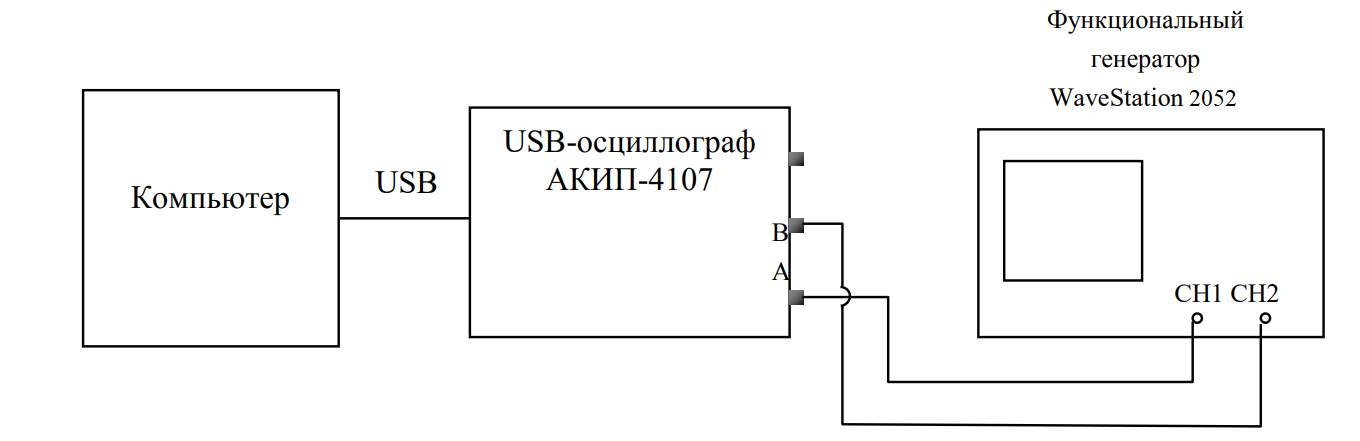
\includegraphics[width=1\linewidth]{scheme}
	\caption{Схема экспериментальной установки}
	\label{fig:scheme}
\end{figure}
Функциональный генератор позволяет сформировать два различных электрических сигнала, которые выводятся на два независимых канала USB-осциллографа.

Инструментальные погрешности считаются малыми.

\equip{Компьютер  с \emph{PicoScope 6}}
\equip{Функциональный генератор \emph{waveStation 2052}}
\equip{USB-осциллограф \emph{АКИП-4108}}

\section{Результаты измерений и обработка данных}

\subsection{Спектры прямоугольных импульсов}

Заметим, что при возрастании $ \tau $ вдвое, ширина спектра уменьшается в 2 раза и в 2 раза возрастает амплитуда спектра.

При увеличении $ f_{повт} = 1/T $ в 2 раза, ширина спектра и $ \delta \nu $ -- частота 1-й гармоники --  увеличивается во столько же раз. 

Изучим зависимость $ \Delta \nu (\tau) $. Результат в таблице \ref{tab:nu-tau}.

\begin{table}[h]
	\centering
	\begin{tabular}{|l|l|l|l|l|l|l|l|l|l|}
		\hline
		${\tau}$      & 40    & 60    & 80    & 100   & 120  & 140  & 160  & 180  & 200  \\ \hline
		${\Delta \nu}$ & 25000 & 17000 & 12500 & 10000 & 8000 & 7000 & 6000 & 5500 & 5000 \\ \hline
	\end{tabular}
	\caption{Зависимость $\Delta \nu (\tau)$}
	\label{tab:nu-tau}
\end{table}

Построим картины спектров для $ \tau  =  50\; мкс $ (рис. \ref{fig:1-50}) и $ \tau = 100\; мкс $ (рис. \ref{fig:1-100}).

\begin{figure}[p]
	\centering
	\includegraphics[width=0.8\linewidth]{"1кгц 50мкс"}
	\caption{Картина спектра прямоугольного сигнала при $\tau = 50$ мкс}
	\label{fig:1-50}
\end{figure}

\begin{figure}[p]
	\centering
	\includegraphics[width=0.8\linewidth]{"1кгц 100мкс"}
	\caption{Картина спектра прямоугольного сигнала при $\tau = 100$ мкс}
	\label{fig:1-100}
\end{figure}

Проверим справедливость соотношения неопределённостей. Построим график $ \Delta \nu (1/\tau) $ на рис. \ref{fig:неопр}; из него видно, что соотношение \eqref{eq:неопр} выполняется с хорошей точностью.

\begin{figure}[tb]
	\centering
	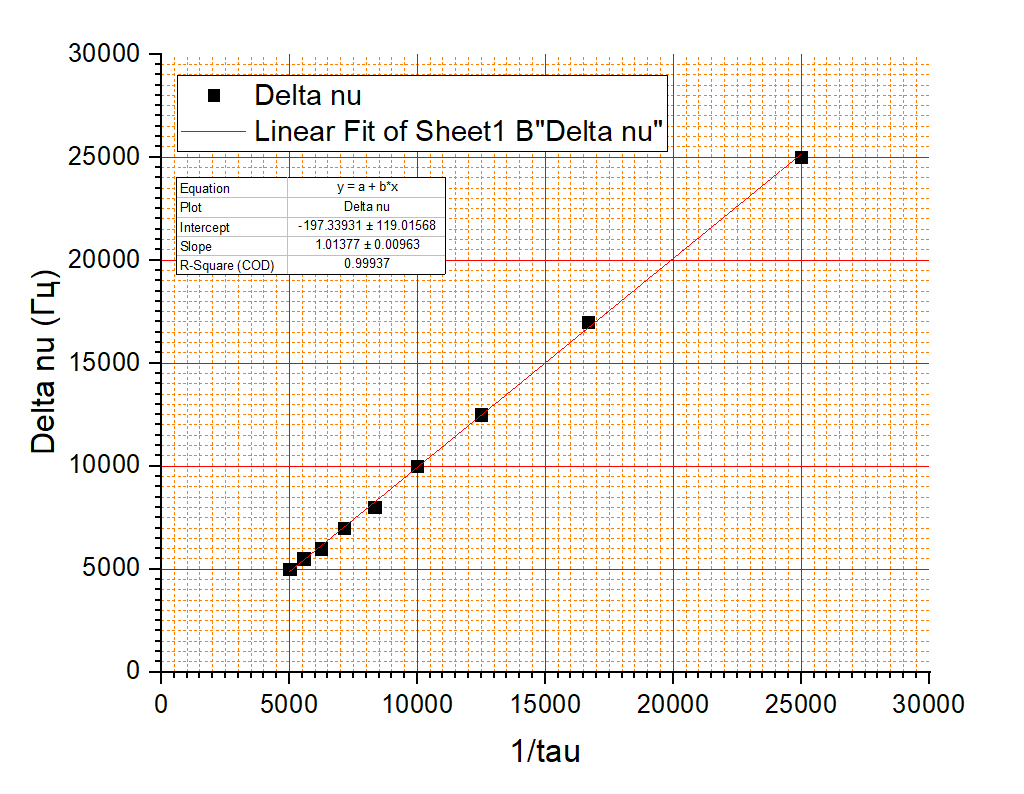
\includegraphics[width=0.8\linewidth]{неопр}
	\caption{График $\Delta \nu (1/\tau)$ для проверки соотношения неопределённостей}
	\label{fig:неопр}
\end{figure}

\subsection{Спектры цугов гармонических  колебаний}

Обратим внимание, что  при увеличении $ \tau $ вдвое ширина спектра убывает, а амплитуда возрастает в 2 раза.

На рис. 8 изображены картины спектра при различных частотах несущей.

Найдём зависимость расстояния между спектральными компонентами $ \delta \nu $ от частоты повторения импульсов $ f_{повт} $. При $f_{повт}  = 0.5, \; 1, \; 2, \; 4, \; 5\; кГц, $ и $ \tau = 100 мкс,  $ выполнено $ \delta \nu = f_{повт}$. Т. к. при проведении эксперимента зависимость снята с недостаточной точностью, нет смысла строить график: угловой к-т при таких данных строго равен 1. Соотношение неопределённостей $ \frac{\delta \nu }{f_{повт}} = \delta \nu \tau  \simeq 1$ выполнено.



\begin{figure}[tbp]
	\centering
	\begin{minipage}{0.8\linewidth}
		\centering
		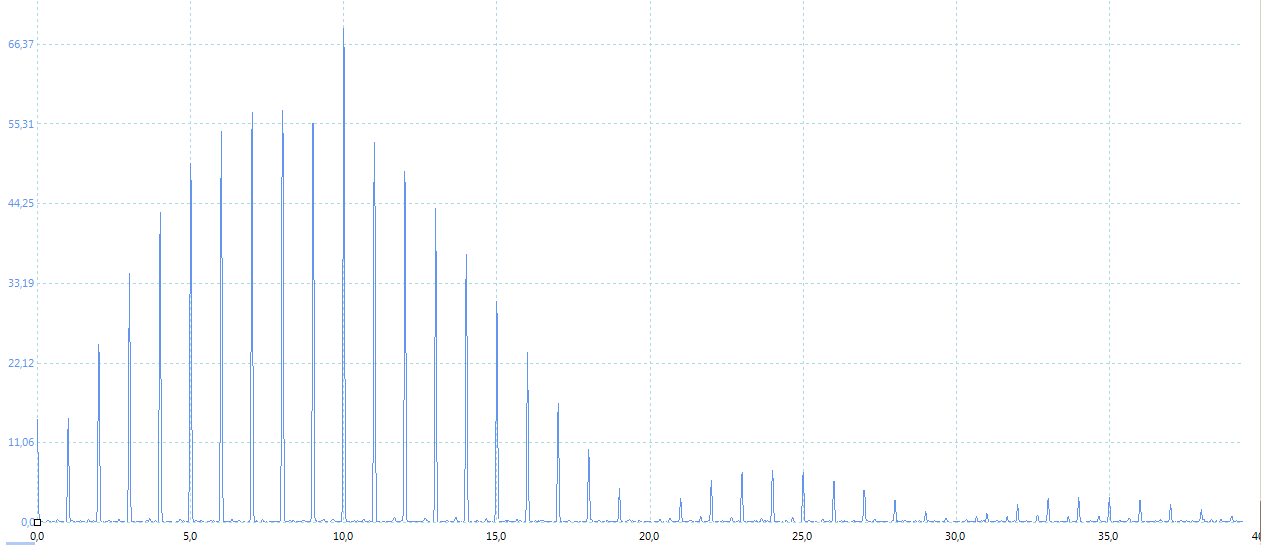
\includegraphics[width=1\linewidth]{Фото/Скрины/3.17(10)}
	\end{minipage}
	\vspace{20pt}	
	
	\begin{minipage}{0.8\linewidth}
		\centering
		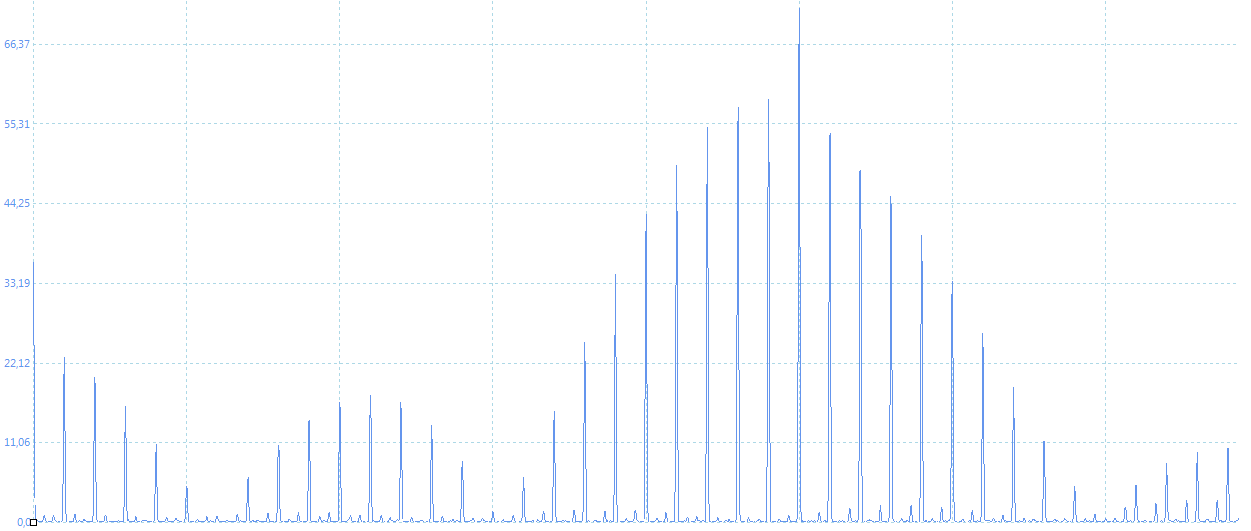
\includegraphics[width=1\linewidth]{Фото/Скрины/3.17(25)}
	\end{minipage}
	\vspace{20pt}
	\label{fig:specr}
	\caption{Картина спектра при $ \nu_0 = 10, \; 25 \;  кГц $}
\end{figure}

Построим картины спектров для $ f_{повт}  = 1\; кГц$ (рис. \ref{fig:1000-hz-zug}) и $ f_{повт}  = 2\; кГц $ (рис. \ref{fig:2000-hz-zug}).

\begin{figure}[p]
	\centering
	\includegraphics[width=0.8\linewidth]{"1000 hz zug"}
	\caption{Картина спектра цугов при $f_{повт} = 1\; кГц$}
	\label{fig:1000-hz-zug}
\end{figure}

\begin{figure}[p]
	\centering
	\includegraphics[width=0.8\linewidth]{"2000 hz zug"}
	\caption{Картина спектра цугов при $f_{повт} = 1\; кГц$}
	\label{fig:2000-hz-zug}
\end{figure}

\subsection{Спектры АМ-сигналов}
\label{punkt}
В табл. \ref{tab:amp} занесены результаты измерения амплитуд сигналов и их гармоник, а также глубину модуляции по формуле \eqref{m}. На основе этих данных построим график $ \frac{U_{min}^s}{U_{max}^s}(m) $ на рис. \ref{fig:-}. Его угловой коэффициент $ k= 0.49 $, что согласуется с теорией, т. к. из \eqref{new}, $ k = 0.5 $. 

Последнее значение существенно выбивается из графика. Видимо, это связано с ошибкой при проведении эксперимента.

\begin{table}[h]
	\centering
	\begin{tabular}{|l|l|l|l|l|l|}
		\hline
		$U_{ch1}$, В & $U_{max}^O$, мВ & $U_{min}^O$, мВ & $U_{max}^S$, мВ & $U_{min}^S$, мВ & $m$    \\ \hline
		0.2          & 546             & 450             & 321             & 15.7            & 0.0964 \\ \hline
		0.5          & 624             & 376             & 321             & 37.9            & 0.248  \\ \hline
		0.8          & 709             & 302             & 322             & 61.9            & 0.402  \\ \hline
		1.2          & 779             & 225             & 322             & 85.0            & 0.552  \\ \hline
		1.5          & 875             & 125             & 322             & 117             & 0.750  \\ \hline
		1.8          & 960             & 58.4            & 322             & 140             & 0.885  \\ \hline
		2            & 998             & 0.00            & 322             & 175             & 1.00   \\ \hline
	\end{tabular}
	\caption{Результаты измерений амплитуд осциллограмм и спектра АМ-сигналов}
	\label{tab:amp}
\end{table}

\begin{figure}
	\centering
	\includegraphics[width=0.8\linewidth]{"бок осн"}
	\caption{Зависимость $U_{min}^s/U_{max}^s$ от глубины модуляции}
	\label{fig:-}
\end{figure}

\subsection{Оценка погрешностей}

Будем считать, что генерируемый источником сигнал имеет высокую точность, а осциллограф -- низкие инструментальные погрешности, поэтому не будем учитывать погрешностей $ \tau $, $ f_{повт} $, $ \nu $, а $ \sigma_\nu $ и $ \sigma_u $ возьмём равными $ \pm 100 $ Гц и $ \pm 0.001 $ В соответственно, т. к. приблизительно такая ошибка измерения по экрану осциллографа. 

Тогда в пп. \ref{punkt} определим погрешность $ m $ по формуле
\begin{equation}\label{key}
	\sigma_m = m \sqrt{\frac{2 \sigma_u^2}{(U_{max}^O+U_{min}^O)^2}+\frac{2 \sigma_u^2}{(U_{max}^O-U_{min}^O)^2}}\approx \frac{m \sqrt{2} \sigma_u}{U_{max}^O-U_{min}^O}, 	
\end{equation}
а погрешность отношения амплитуд найдём через
\begin{equation}\label{key}
	\sigma_{\frac{U^S_{min}}{U^S_{max}}} = \frac{U^S_{min}}{U^S_{max}} \sqrt{\frac{\sigma_u^2}{(U_{min}^S)^2}+\frac{\sigma_u^2}{(U_{max}^S)^2}},
\end{equation}
и учтём их при построении графика.
\section{Вывод}
Провели исследование нескольких типов периодических сигналов; исследовали их разложение в гармонический спектр, получили картины спектров. Проверили справедливость нескольких соотношений, в том числе формулы \eqref{eq:неопр}.
\newpage
\begin{thebibliography}{9}
\bibitem{Siv} Сивухин Д. В. \emph{Общий курс физики. Том 3 Электричество и магнетизм}, 2004
\bibitem{kirich} Кириченко Н.А. \emph{Электричество и магнетизм.}, 2011
\bibitem{max} \emph{Лабораторный практикум по общей физике. В 3 томах. Том 2. Электричество и магнетизм: учебное пособие} под ред. А. В. Максимычева, М. Г. Никулина
\end{thebibliography}
\end{document}

